\documentclass[a4paper,10pt,oneside]{article}
\usepackage{graphicx}
\usepackage{color}
\usepackage{url}
\usepackage{subfigure}
\usepackage[utf8]{inputenc}
\usepackage[T1]{fontenc}
\usepackage{tgpagella}
%\usepackage[scale=0.9]{tgcursor}
%\usepackage[scale=0.9]{tgheros}
\usepackage{xstring}

\newcommand{\myscale}{0.74}
\newcommand{\vect}[1]{\boldsymbol{#1}}
\newcommand{\code}[1]{\texttt{\StrSubstitute{#1}{.}{.\.}}}
\def\.{\discretionary{}{}{}}
\newcommand{\jmodule}[1]{\emph{#1}}

\setlength{\hoffset}{-1in} %left margin will be 0, as hoffset is by default 1inch
\setlength{\voffset}{-1in} %analogous voffset
\setlength{\oddsidemargin}{1.5cm}
\setlength{\evensidemargin}{1.5cm}
\setlength{\topmargin}{1.5cm}
\setlength{\textheight}{24cm}
\setlength{\textwidth}{18cm}

\def\mftitle{jInfer Architecture}
\def\mfauthor{Michal Klempa, Mário Mikula, Robert Smetana, Michal Švirec, Matej Vitásek}
\def\mfadvisor{RNDr. Irena Mlýnková, Ph.D., Martin Nečaský, Ph.D.}
\def\mfplacedate{Praha, 2011}
\title{\bf\mftitle}
\author{\mfauthor \\ Advisors: \mfadvisor}
\date{\mfplacedate}

\ifx\pdfoutput\undefined\relax\else\pdfinfo{ /Title (\mftitle) /Author (\mfauthor) /Creator (PDFLaTeX) } \fi

\begin{document}
\maketitle
\noindent Target audience: developers willing to extend jInfer.

\noindent\emph{Note: we use the term \textbf{inference} for the act of creation of schema throughout this and other jInfer documents.}\\

The description of jInfer architecture will be divided into 3 main views: the data view, the process view and the plaform view.
The data view will commence by describing the data structures, namely representations of regular expressions and XML elements, attributes and simple data. The notions of a \emph{rule} and a \emph{grammar} will be explained, along with the finite state automata representation we use.

Afterwards the process of inference will be described, both from high-level and programmatic point of view.
Finally, we will look at jInfer as at an NetBeans Platform application consisting of a number of modules performing their tasks and communicating together through a set of well-defined interfaces.

\section{Package naming conventions}
All packages start with \code{cz.cuni.mff.ksi.jinfer}. Afterwards is the short, normalized name of the NetBeans module (e.g. \code{base}) and finally the package structure in this module (e.g. \texttt{objects.utils}). All in all, a package in the \jmodule{Base} module could look like \code{cz.cuni.mff.ksi.jinfer.base.objects.utils}.

\section{Data view}
\subsection{Regular expressions}
For general information on regular expressions, please refer to \cite{wikiregexp}, \cite{automatatheory}.
All classes pertaining to regular expressions can be found in the package \code{cz.cuni.mff.ksi.jinfer.base.regexp}.
In jInfer, we use extended regular expressions as they give us nicer syntax (and easier programming).

Regular expression is implemented as class \code{Regexp<T>} with supporting classes \code{RegexpInterval} and \code{Reg\.exp\.Type}.
Each \code{Regexp<T>} instance has a type of \code{RegexpType} enum.
\begin{itemize}
	\item Lambda ($\lambda$) - empty string (also called $\epsilon$ in literature).
	\item Token - a letter of the alphabet.
	\item Concatenation - one or more regular expression in an ordered sequence. Eg. $(a, b, c, d)$.
	\item Alternation - a choice between one or more regular expressions. Eg. $(a | b | c | d)$.
	\item Permutation - shortcut for all possible permutations of regular expressions. Our notation is $(a\& b\& c\& d)$.
\end{itemize}
Type of regexp is in \code{type} member in class \code{Regexp<T>} and can be tested by calling methods \code{isLa\.mb\.da()}, \code{isTo\.ken()}, \code{isCon\.ca\.te\.na\.tion()}, \code{isAlt\.er\.na\.tion()}, \code{isPer\.mu\.ta\.tion()}.

Each \code{Regexp<T>} instance has one instance of \code{RegexpInterval} as member.
Class \code{RegexpInterval} represents POSIX-like intervals for expression.
\begin{itemize}
	\item $a\{m,n\}$ means $a$ at least $m$-times, at most $n$-times.
	\item $a\{m,\}$ means at least $m$-times (unbounded).
\end{itemize}
Interval can be either bounded (you have to set both lower and upper bound integers), or unbounded (you have to set only lower bound).
Testing interval value commonly follows this routine.
\begin{verbatim}
RegexpInterval i = r.getInterval();
if (i.isUnbounded()) {
  print(i.getMin());
} else {
  print(i.getMin(), i.getMax());
}
\end{verbatim}
That is, first check interval for being unbounded, only if it is bounded, you can ask for maximum.

Using Java generics, \code{Regexp<T>} can represent regular expression over any alphabet.
Only token regexps actually hold instance of type \code{T} in member \code{content}.

Regular expression is in fact $n$-ary tree, for example expression $(a, b, ((c | d), e), f)$ can be viewed as in fig. \ref{reg_tree}.
\begin{figure}
\centering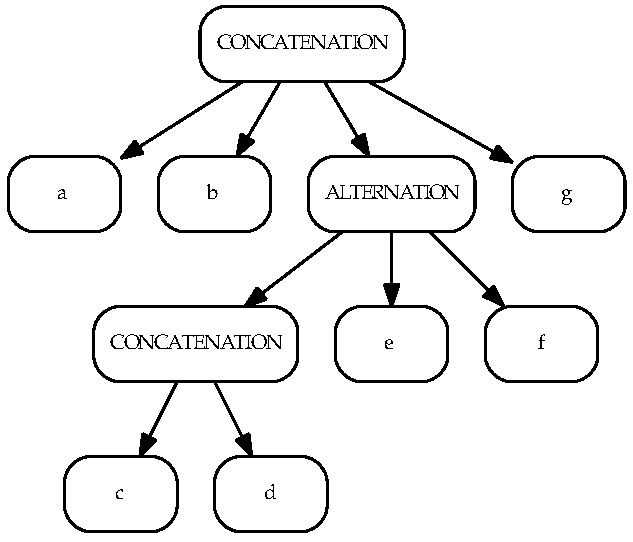
\includegraphics[scale=\myscale]{reg_tree}
\caption{Example tree for regular expression $(a, b, ((c | d), e), f)$} \label{reg_tree}
\end{figure}
We implement this tree in a member of \code{Regexp<T>} class called \code{children}, which is of type \code{List<Regexp<T>{}>}.
List contains children of regexp: a node contains a list of child nodes in the tree view.

Regexp has to obey the following constraits.
\begin{itemize}
	\item Type, children and interval have to be non-\code{null} references.
	\item When type is lamba, content and interval has to be \code{null}.
	\item When type is token, content has to be non-\code{null}.
	\item When type concatenation, alternation or permutation, content has to be \code{null}.
\end{itemize}
These constraits are checked by constructors, therefore the best way to construct new regexps is by using methods \code{get\.To\.ken(), get\.Con\.ca\.te\.na\.tion()} etc.

For these cases, special \code{getMutable()} method is implemented to obtain regexp with none of the members set. One has to fill in all properties carefully and call \code{setImmutable()} aftewards. Proper usage should be one of following: % TODO anti WTF?
Regexp instance is by default created as immutable, that is, once instantiated, you cannot add more children to list of children, cannot change type, content etc. In special circumstances, one does not know future children of regexp at the time of creation. This occurs mainly in input modules: while parsing XML data sequentially, one does not know contents of element in time of handling start element event.
\begin{verbatim}
	Regexp<T> r = Regexp.<T>getMutable();
	r.setInterval(...);
	r.setType(RegexpType.LAMBDA);
	r.setImmutable();cz.cuni.mff.ksi.jinfer.base
\end{verbatim}
\begin{verbatim}
	Regexp<T> r = Regexp.<T>getMutable();
	r.setInterval(...);
	r.setType(RegexpType.TOKEN);
	r.setContent(...)
	r.setImmutable();
\end{verbatim}
\begin{verbatim}
	Regexp<T> r = Regexp.<T>getMutable();
	r.setInterval(...);
	r.setType(RegexpType.CONCATENATION);
	r.addChild(...);
	r.addChild(...);
	r.addChild(...);
	r.setImmutable();
\end{verbatim}
	
Finally, regexp contains a useful method to obtain all leaves in the regexp tree. It is called \code{getTokens()} and it recursively traverses tree returning list of leaves (token type regexps).

\subsection{XML representation}
XML data basically encompasses elements, text nodes (characters inside elements) and attributes.
For maximum generality, we decided to break apart these objects.
We define three basic interfaces: \code{NamedNode}, \code{StructuralNode} and \code{ContentNode} (see package \code{cz.cuni.mff.ksi.jinfer.base.interfaces.nodes}). 

The first stands for a bare node in XML document tree, it has its name and context within the tree (path from root).
The latter two extend \code{NamedNode} interface.
\code{StructuralNode} is for nodes which form structure of XML document tree: elements and text nodes.
\code{ContentNode} is for nodes that have content in XML documents: text nodes and attributes.
We have three classes: \code{Element} for elements, \code{SimpleData} for text nodes, \code{Attribute} for attributes (see package \code{cz.cuni.mff.ksi.jinfer.base.objects.nodes}).
In theory, the classes and interfaces would be layed out as in fig. \ref{interfaces_nodes}
\begin{figure}
\centering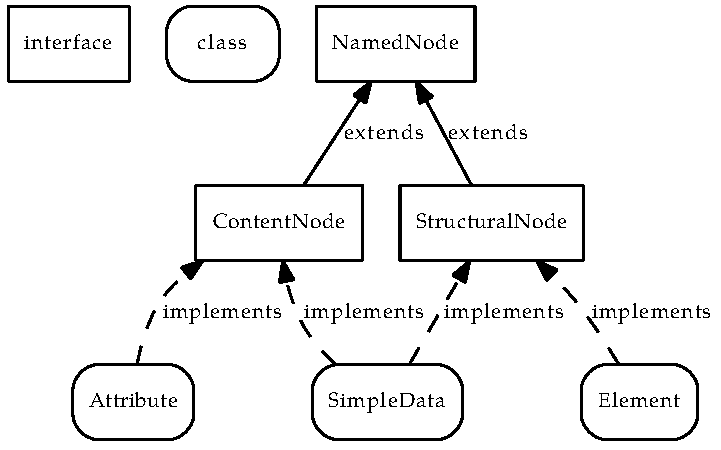
\includegraphics[scale=\myscale]{interfaces_nodes}
\caption{How should interfaces and classes for XML representation look like in theory} \label{interfaces_nodes}
\end{figure}
\begin{figure}
\centering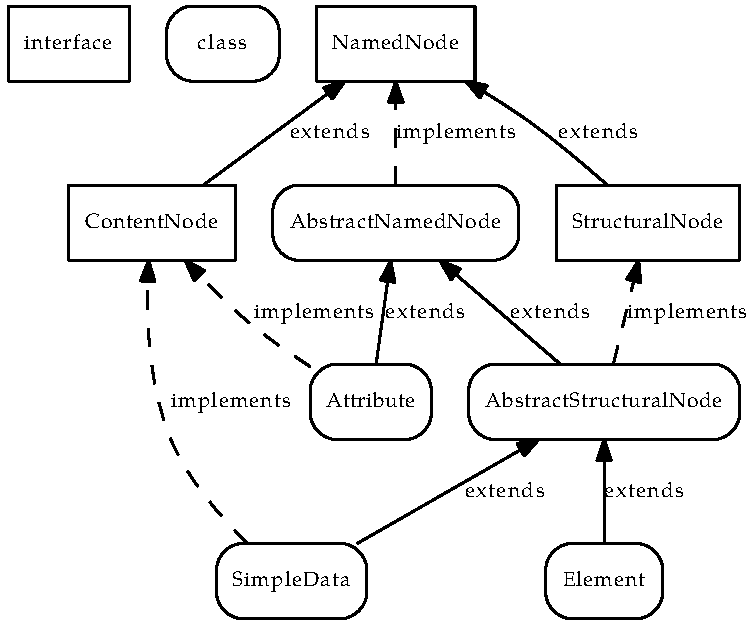
\includegraphics[scale=\myscale]{nodes}
\caption{How are interfaces and classes for XML representation arranged in practice} \label{nodes}
\end{figure}
% This figure has been replaced by UML-like
%\begin{figure}
%\centering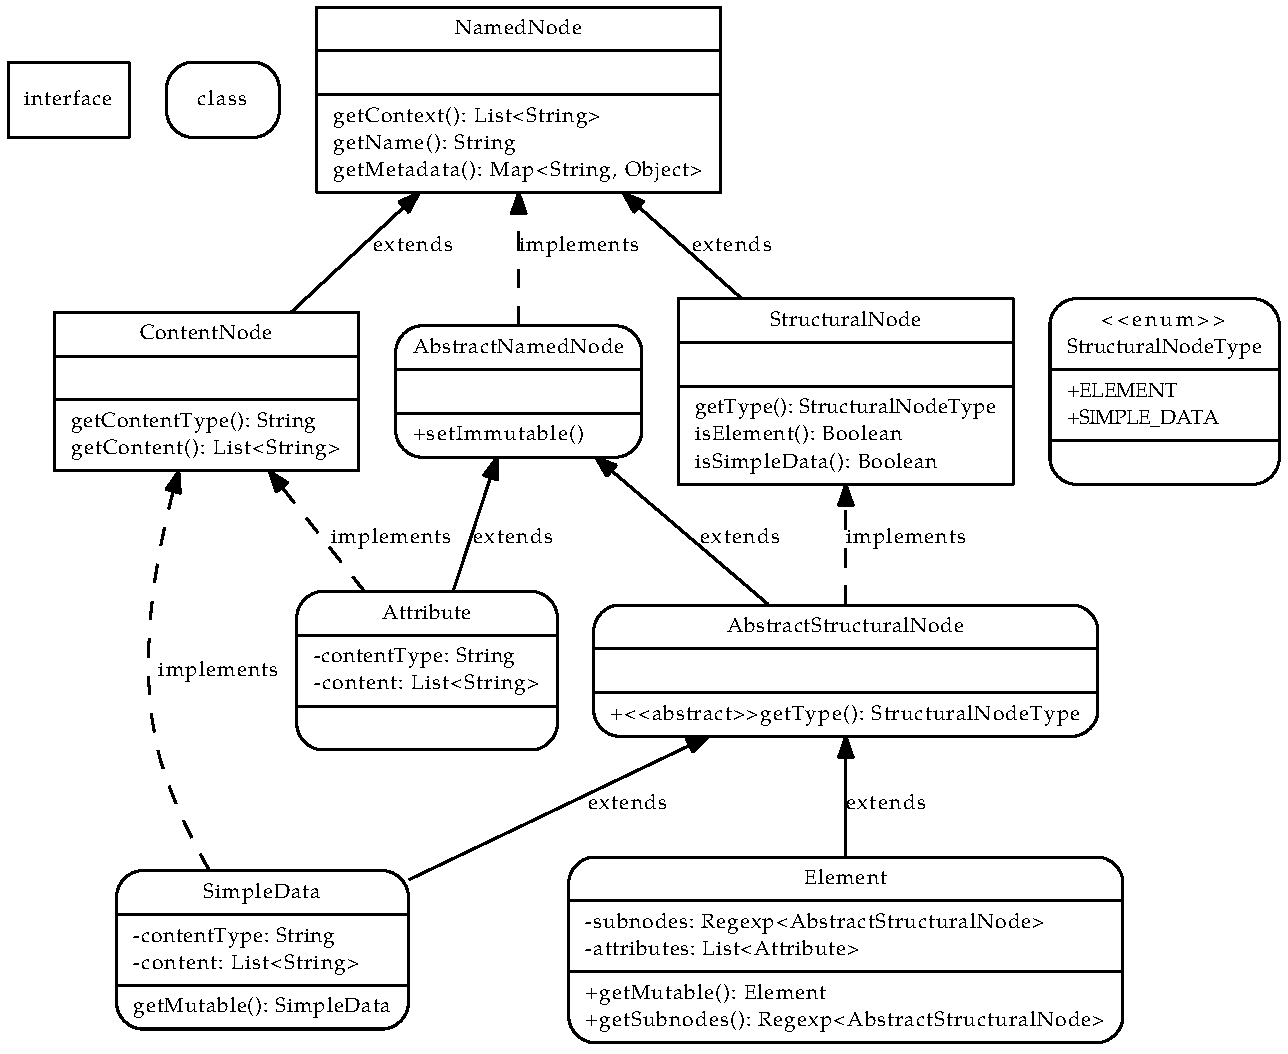
\includegraphics[scale=\myscale]{nodes_full}
%\caption{XML representing interfaces and classes in detail} \label{nodes_full}
%\end{figure}
\begin{figure}
\centering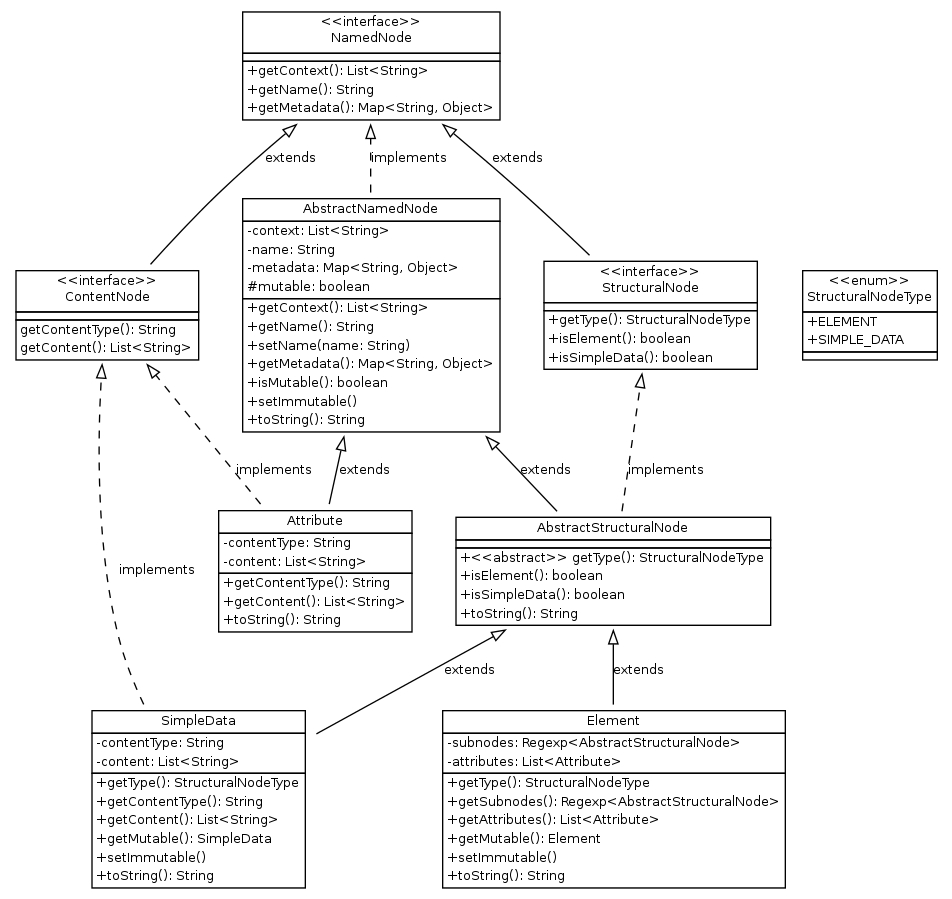
\includegraphics[scale=\myscale]{nodes_full2}
\caption{Class diagram for XML representing interfaces and classes} \label{nodes_full2}
\end{figure}

For even more generality in design, we decided to implement abstract classes in midlevel:
\begin{itemize}
	\item \code{AbstractNamedNode} which implements methods from \code{NamedNode} interface to handle context, name and metadata (will discuss later in section \ref{section_metadata}),
	\item \code{AbstractStructuralNode} which implements only the task of deciding if instance is \code{Element} or \code{SimpleData}.
\end{itemize}
On the one hand, we are interested in the XML structure - for this reason we use \code{isElement()} and \code{isSimpleData()} of \code{AbstractStructuralNode}. On the other hand, we want to access textual content and its type, for this reason we use \code{getContent()} and \code{getContentType()} of \code{ContentNode}.

Finally, our interface/class model for representing XML nodes is drafted in fig. \ref{nodes}. Those who are brave enough can look at fig. \ref{nodes_full2}.

Class \code{Element} has two important members.
\begin{itemize}
	\item \code{Regexp<AbstractStructuralNode> subnodes} - representing the right side of a grammar rule,
	\item \code{List<Attribute> attributes} - representing all attributes in this element.
\end{itemize}
These two are filled in by import modules, processed further by inference (simplification) modules and finally exported by schema generator modules.

As in regular expressions, classes pertaining to XML nodes are by default immutable.
For elements, it means no adding of attributes and changing regexp reference (regexp instance itself is immutable as well).
The same \code{getMutable()} principles and good usage practises hold for these classes.

\begin{figure}
\centering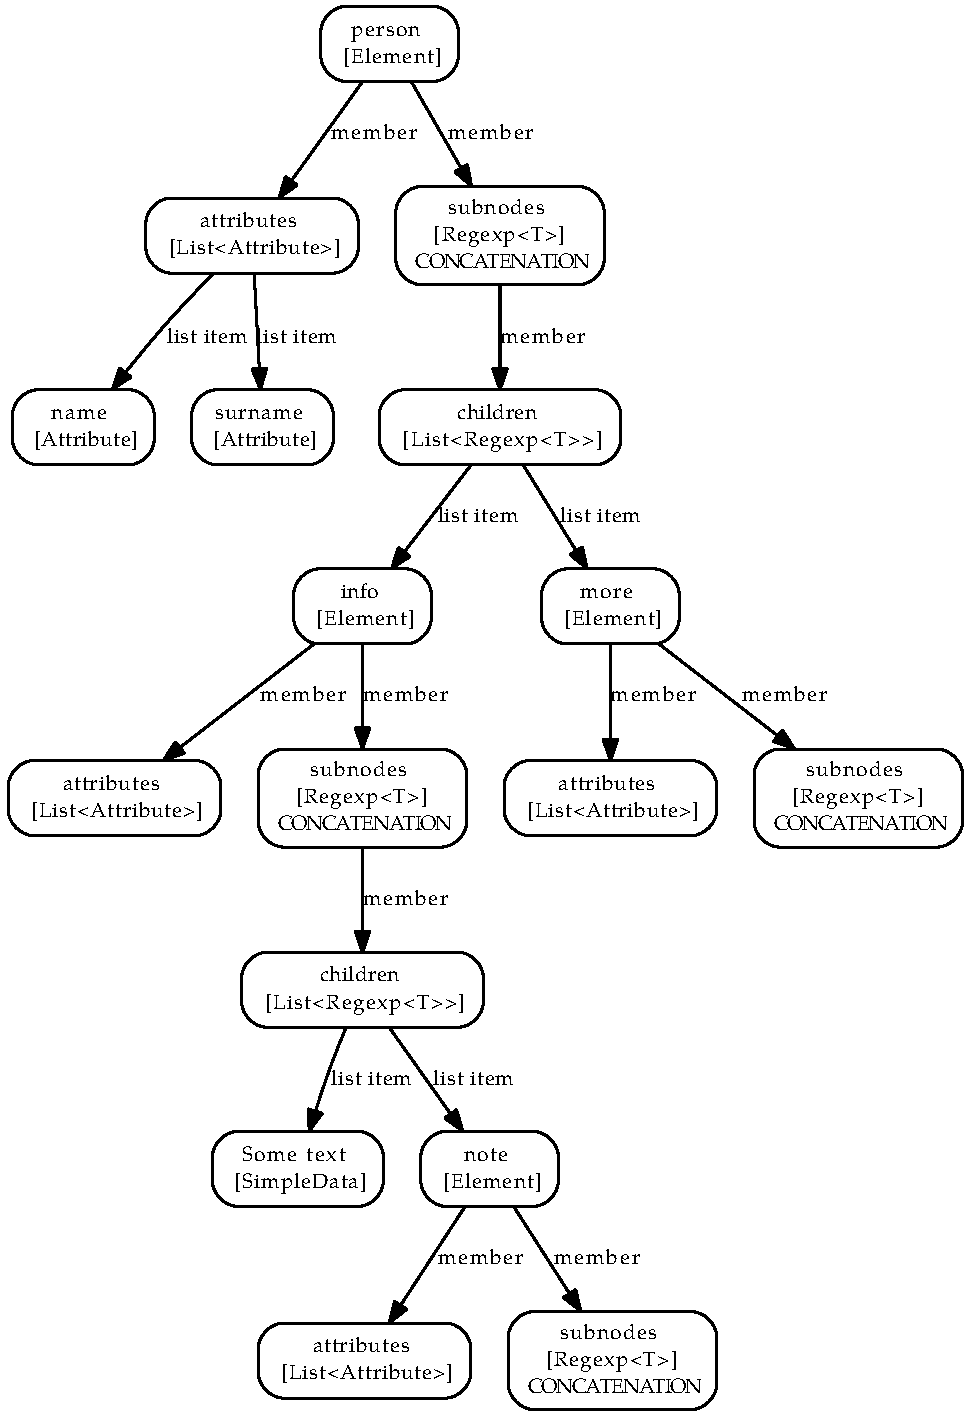
\includegraphics[scale=\myscale]{xml_example}
\caption{XML document representation} \label{xml_example}
\end{figure}
Let's have an example: the following XML document would be represented as tree in fig. \ref{xml_example}.
\begin{verbatim}
  <person name="john" surname="smith">
    <info>
      Some text
      <note/>
    </info>
    <more/>
  </person>
\end{verbatim} 
Although in example we present the whole document tree, input modules produce slightly different format (consisting of rules).

\subsection{Rules and grammars} \label{rules_grammar}
jInfer and its documentation use extended context-free grammars\cite{extendedcfg}.
\emph{Rules} in such grammar are in the form
$$
  \textnormal{Left Hand Side (LHS)} \to \textnormal{Right Hand Side (RHS)}
$$
where LHS is a letter of the alphabet (token), RHS is a regular expression over this alphabet. Example would be
$$
  a \to b, (c | d)\ast
$$
In jInfer each such rule is represented with an \code{Element} instance. In this representation, the \code{Element} itself is the LHS, its \code{subnodes} are the RHS.

Another important notion is a \emph{grammar}. A grammar consists of its rules, so in jInfer a grammar is just a collection of \code{Element}s. Closely related term is \emph{Initial Grammar}, which for us is a grammar consisting of rules with \emph{simple} right hand sides, i.e. just concatenations of tokens (even with no children, see fig. \ref{xml_example} again). Initial Grammar is produced by \jmodule{Initial Grammar Generator}.

\subsection{Nondeterministic Finite Automaton}
We recommend skipping this section during the first reading as it describes advanced features.

For all inference algorithms based on merging states of NFA's, our implementation of nondeterministic finite automaton might be interesting.
Implementation consists of 4 classes (see package \code{cz.cuni.mff.ksi.jinfer.base.automaton}).
\begin{itemize}
  \item \code{Automaton<T>}
  \item \code{Step<T>}
  \item \code{State<T>}
  \item \code{AutomatonCloner<A, B>}
\end{itemize}
The implementation uses Java generics to represent symbol of alphabet.
We denote \code{T} the Java type of that symbol.

Automaton uses \code{equals()} to compare symbols on transitions (when building prefix-tree automaton and when merging states).
If you are using strings, you're just fine. With complicated objects, the first option is to make sure that equivalent objects are properly tested in \code{equals()}.
Second, maybe faster solution is to cluster objects into classes of equivalence before inserting them into automaton.
Then give automaton only cluster representant object (which will use java \code{Object.equals()} with reference comparison) for each object encountered.

\paragraph{State}
Let's begin with the smallest of classes, the \code{State<T>}.
It represents automaton state, it has two integer members: \code{name} and \code{finalCount}.
Name clearly serves as name of state in visualization and to-string conversion.
Final count is for representing whether the state is final in automaton.
The field is not true/false but integral to help algorithms use statistics over automatons (how many times in XML input is this state final?).

\paragraph{Step}
Next we have \code{Step<T>} which stands for automaton transition.
It has its \code{source} and \code{destination} states references.
Symbol accepted by using this transition is stored in \code{acceptsSymbol} member of generic type \code{T}.
And finally member \code{useCount}, which is integer stating how many times the transition was used when constructing prefix tree automaton from input data.
Simplifying algorithm can use this number for statistic purposes.

\paragraph{Automaton}
\code{Automaton<T>} class puts these together to form a nondeterministic finite automaton.
It has reference to \code{initialState}, it has \code{newStateName} integer value to assure unique state names inside one automaton (incrementing every time new state is created).
We use two maps to implement transition function ($\delta$-function).
One map of type \code{Map<State<T>, Set<Step<T>{}>{}>} called \code{delta} represents mapping from state into set of all outgoing transitions from state.
Second is just reversed map, called \code{reverseDelta}, which holds all incoming transitions into state (for better performance).
There is only one instance of each step from one state to another.
That instance is referenced in delta map (on place of source state) and in reverse delta map (on place of destination state).
Loops are no speciality, only source = destination.

Automaton supports creation as a copy of another one (not reference copy, but deep copy expect of symbols), this can be used when searching solution space to create more versions of automaton to edit.
We implemented building of prefix-tree automaton (PTA) in \code{buildPTAOnSymbol()} method.
Create empty automaton and then call this method for every input string of language.
You will get PTA with useCounts and finalCounts set properly on steps/states.
\begin{figure}
	\centering
	\subfigure[Before merge.]
	{
		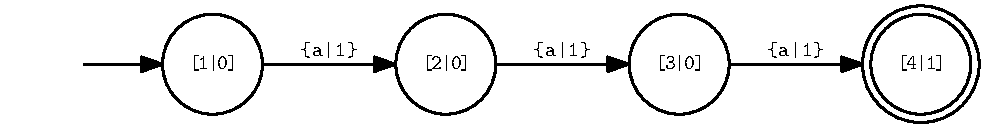
\includegraphics[scale=\myscale]{automaton_merge1}
		\label{automaton_merge1}
	}
	\subfigure[After states 3 and 4 merged.]
	{
		\centering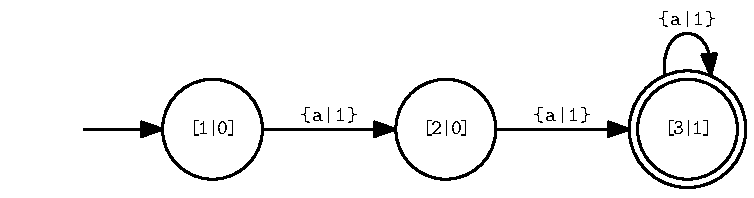
\includegraphics[scale=\myscale]{automaton_merge2}
		\label{automaton_merge2}
	}
	\subfigure[After states 2 and 4 merged.]
	{
		\centering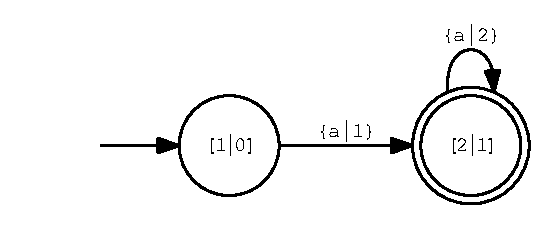
\includegraphics[scale=\myscale]{automaton_merge3}
		\label{automaton_merge3}
	}
	\caption{Sample automaton.} \label{automaton_merge}
\end{figure}
The biggest thing we offer to researchers is state merging by simply calling \code{mergeStates(state1, state2)} method.
Method merges second state given into first one (or an overloaded version - all states in list into first one in list).
All \{in|out\}-transitions are redirected properly (or discarted as needed).
Variables \code{useCount} and \code{finalCount} are updated to sums of values from merged transitions/states.

To be able to refer to states that have already been merged (and thus have a different name), we use a map of renamings.
Lets take example automaton of fig. \ref{automaton_merge1} (states are labeled [name|finalCount], steps by \{symbol|useCount\}).
One asks to merge states 3 and 4.
State 3 then becomes final state with loop and state 4 disappears (fig. \ref{automaton_merge2}).
If then one asks to merge states 2 and 4, automaton properly handles situation by knowing, that old state 4, was merged into state 3, and merges states 2 and 3 (see fig. \ref{automaton_merge3}).
This can be useful in $k,h-context$ and $s,k-strings$ implementations (find all context/strings, then supply list of states to merge and don't bother with state names updates).

\paragraph{AutomatonCloner}
Class \code{AutomatonCloner<A, B>} has one overloaded method \code{convertAutomaton()}.
First version accepts automaton and class implementing \code{AutomatonClonerSymbolConverter<A, B>} interface, and returns new automaton with same structure, but with symbols on transitions from alphabet of Java type \code{B}.
Second version takes two automatons, second one has to be empty (without initial state created), and symbol converter.
It fills in second automaton to have same structure as first one, but with symbols of type \code{B}.

To fulfil symbol conversion, one have to provide implementation of \code{AutomatonClonerSymbolConverter<A, B>} interface.
Interface has one method.
\begin{verbatim}
	B convertSymbol(final A symbol);
\end{verbatim}
Its purpose is to provide mapping from symbol over one domain to new symbols.
Implementation has to be \code{equals()} consistent, if in first automaton are two transitions with symbols \code{a}, \code{b} such that
\code{a.equals(b) == true}, converter has to produce new symbols that are equal.

\section{Process view} \label{section_inference_process}
\begin{figure}
	\centering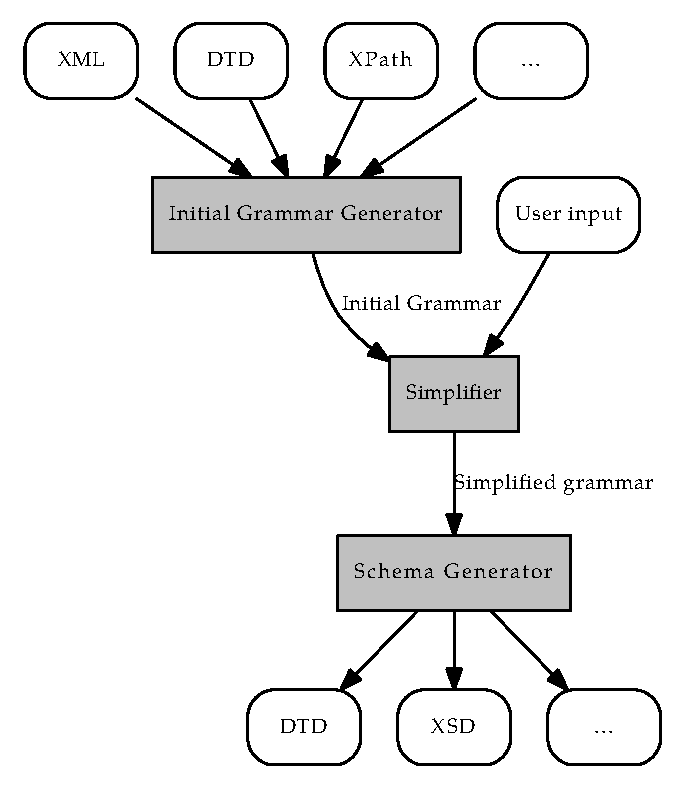
\includegraphics[scale=\myscale]{inference_process}
	\caption{High-level view of the inference process} \label{inference_process}
\end{figure}
The process by which jInfer infers the resulting schema from various inputs (inference process) is summarized by fig. \ref{inference_process}. From the high-level viewpoint, it consists of three consecutive steps carried out by three different modules:
\begin{enumerate}
	\item Initial Grammar (IG) generation: done by the \jmodule{Initial Grammar Generator (IGG)} module, this is the process of converting all of the inputs to IG representation. All documents, schemas and queries selected as input are evaluated, simple rules are extracted and in the end sent to the next step.\\
	For example, a trivial XML document
	\label{example_inference_xml}
	\begin{verbatim}
<person name="john" surname="smith">
  <info>
    Some text
    <note/>
  </info>
</person>
<more/>
<person>
  <more/>
  <more/>
  <more/>
</person>
  \end{verbatim}
	will translate into the following IG rules
	\begin{eqnarray*}
		person & \to & \mathit{info}, more, more, more, more \\
		\mathit{info} & \to & simple\_data, note \\
		note & \to & empty\_concatenation \\
		more & \to & empty\_concatenation \\
		person & \to & more, more, more \\
		more & \to & empty\_concatenation \\
		more & \to & empty\_concatenation \\
		more & \to & empty\_concatenation \\
	\end{eqnarray*}
	\item Simplification: done by the \jmodule{Simplifier} module, this is the process of simplifying, compressing or somehow compactly describing the IG by a smaller number of (more complex) rules (exactly one rule for each element). User interaction might be used in this step to help achieve better simplification. At the end of this step, all rules are sent to the export step.\\
	For example, previous rules for element person could be simplified to a single rule
	\begin{eqnarray*}
		person & \to & \mathit{info}?, more\{1, 3\}
	\end{eqnarray*}
	Rules for elements info, more and note after simplification will be:
	\begin{eqnarray*}
		\mathit{info} & \to & simple\_data, note \\
		note & \to & \lambda \\
		more & \to & \lambda
	\end{eqnarray*}
	Note the lambda regular expressions for note and more. In Initial Grammar, all regexps are concatenations (even empty), but in simplified grammar, if element have to be empty in schema, it has to have lambda regular expresion as subnodes.	
	\item Schema export: done by the \jmodule{Schema Generator (SchemaGen)} module, this is the process of actually creating the resulting schema file from the simplified rules. Result of this step is a string representation of the schema, which is sent back to the framework (and later displayed, saved, etc).\\
	For previous simplifier rules, the resulting DTD would be:
	\begin{verbatim}
	<!ELEMENT person (info?, more, more?, more?)>
	<!ELEMENT info (#PCDATA | note)*>
	<!ELEMENT note EMPTY>
	<!ELEMENT more EMPTY>
	+ attributes
	\end{verbatim}
	For element person, even when simplified grammar specifies its occurence to at least once, at most 3 times, as DTD has no such construct, export module have to do some magic. Situation is even worse for elements that contain simple data inside simplified rule. Only way to express mixed content in DTD is to use \verb.(#PCDATA | note)*. construct. Even if regular expression is complicated, export module has to do this "flattening".texmaker
	Lets look on XSD output of same rules:
	\begin{verbatim}
	<xs:element name="person">
	  <xs:complexType>
	    <xs:sequence>
	      <xs:element name="info" minOccurs="0" maxOccurs="1">
	        <xs:complexType mixed="true">
	          <xs:sequence>
	            <xs:element name="note" minOccurs="1" maxOccurs="1">
	              <xs:complexType>
	              </xs:complexType>
	            </xs:element>
	          </xs:sequence>
	        </xs:complexType>
	      </xs:element>
	      <xs:element name="more" minOccurs="1" maxOccurs="3"/>
	        <xs:complexType>
	        </xs:complexType>
	      </xs:element>
	    </xs:sequence>
	  </xs:complexType>
	</xs:element>
	+attributes
	\end{verbatim}
\end{enumerate}
Important thing to note here is that all these steps are executed consecutively. That means, \jmodule{Simplifier} is only started \emph{after} the \jmodule{IGG} completely finished its work and returned IG to be simplified. Similarly, \jmodule{SchemaGen} gets all the rules to export at once, in one list.

This modular architecture means that it is possible to replace any and/or all of these modules with \emph{something} else that does similar job. In practice, researchers will probably implement new \jmodule{Simplifier} modules, while using our implementation of BasicIGG and export modules. This modular scheme is also used inside our modules to divide them into submodules. It is possible to add new file format processing to import/export. One can extend automaton merging state algorithm of our implementation of \cite{ahonen} in TwoStepSimplifier module by replacing submodules. % TODO anti This is a terrible paragraph with no clear path to follow, please reorganize (sentences on their own are OK)

\subsection{Programmatic view}
From developer's point of view, inference modules are just properly annotated classes (see \ref{section_lookups}) implementing one of the following interfaces (all found under \code{cz.cuni.mff.ksi.jinfer.base.interfaces.inference})
\begin{itemize}
	\item \code{IGGenerator}
	\item \code{Simplifier}
	\item \code{SchemaGenerator}
\end{itemize}
A nice way to name such a class is by adding \code{-Impl} to the name of implemented interface, for example \code{Sim\.pli\.fier\.Impl}.
Annotation required for the framework to recognize such a class as an inference module is the following
\begin{verbatim}
	@ServiceProvider(service = <interface>.class)
\end{verbatim}
for example
\begin{verbatim}
	@ServiceProvider(service = Simplifier.class)
\end{verbatim}
The most important method in each module is \code{start}, defined in each of the interfaces. This method is called by the framework when the respective step of inference is to be executed. It has always two parameters: the actual input data for the module, and a callback object to report to when this step is finished. We will look at both parameters now in more detail. 

\subsubsection{Module input}
Each inference module takes the actual input data as the first parameter of its \code{start} method. The type of the argument differs based on the inference module.

\jmodule{Simplifier} and \jmodule{Schema Generator} take grammar (see \ref{rules_grammar}), in other words a list of \code{Element}s as input. In the first case, this grammar is the Initial Grammar, in the second case it is the simplified grammar.

\jmodule{Initial Grammar Generator} takes an object of type \code{Input}. This class encapsulates all the input files in 3 collections of \code{File}: \code{documents}, \code{schemas} and \code{queries}. Enumerating these files provides IGG with access to all data it needs to create Initial Grammar.

\paragraph{Initial Grammar} has two formats:
\begin{itemize}
	\item \textbf{Only concatenations.} This is the default format. All regular expressions coming from IGG have to be concatenations, even if they are empty.
	When importing XML documents this is just fine, because a document is a positive example of language we are trying to identify.
	But while importing schemas, queries or other stuff that can contain more information, it might be necessary to convert it somehow to concatenations.
	For example, when importing DTD:
	\begin{verbatim}
	<!ELEMENT person (info?, more, more?, more?)>
	<!ELEMENT info (#PCDATA | note)*>
	<!ELEMENT note EMPTY>
	<!ELEMENT more EMPTY>
	\end{verbatim}
	% TODO anti Emphasise elements in the following paragraph
	Elements note and more are empty, but we cannot use lambda regexp. Import will use empty concatenation instead.
	For element person, import module has to generate some positive examples of language generated by regular expression \verb+(info?, more, more?, more?)+.
	
	This is basically done by calling \code{cz.cuni.mff.ksi.jinfer.base.interfaces.Expander} interface method \code{expand()}. One can implement own intelligent expander, or use our provided\\ \code{cz.cuni.mff.ksi.jinfer.basicigg.expansion.ExpanderImpl}.
	
	\item \textbf{Complex regular expressions.} Simplifier module running in current inference can indicate support for this format by declaring capability \code{Capabilities.CAN\_HANDLE\_COMPLEX\_REGEXPS}.
	Even then, import module is not obliged to use it of course. But it is reasonable to do so, if imported file type gives more information than simple concatenations (when importing schemas).
	
	Initial Grammar can contain all regular expressions. If schema defines empty element, make its subnodes lambda regexp. If schema defines element content as \verb.(a, b){2,7}(c | d)., just construct that regexp. Empty concatenations are also allowed - as they are positive examples in XML document input. It is simplifier's responsibility to divide rules by import file formats (by using metadata described in \ref{section_metadata}) and to handle empty concatenations from XML file import with complex regular expressions from other formats.
\end{itemize}
If you are writing import module, check if you can provide more information to simplifier from input file type by using complex format.
This interface division allows us to plug in old methods (accepting only XML input) to the chain of inference, even with schema input files.
It may be useful for method benchmarking too.

\paragraph{Simplified grammar} has only one format and that is \textbf{strict regular expression format}. Empty concatenations, alternations or permutations are not allowed. If element should be exported as empty, use lambda regexp as its subnodes.

\subsubsection{Module output}
Second parameter of each inference module's \code{start} method is a callback object. There are 3 callback interfaces defined in the \code{cz.cuni.mff.ksi.jinfer.base.interfaces.inference} package
\begin{itemize}
	\item \code{IGGeneratorCallback}
	\item \code{SimplifierCallback}
	\item \code{SchemaGeneratorCallback}
\end{itemize}
Each callback interface naturally belongs to the similarly named module interface. As their respective interfaces, also callbacks define one crucial method: \emph{finished}. Each inference module is responsible for invoking this method on the callback it got as a parameter, after it has finished its work and has results to be passed on. Again, these 3 finished methods have different arguments based on the inference module.

\code{IGGeneratorCallback.finished()} and \code{SimplifierCallback.finished()} have a grammar (Initial Grammar in case of IGG) as their only argument.

\code{SchemaGeneratorCallback.finished()} has two \code{String}s as arguments: \code{schema} is the actual string representation of the resulting schema, \code{extension} is a file extension of the result (such as "dtd" or "xsd") which the framework will use when saving the result in a file.

\subsubsection{Error handling}
Because the run of each inference module is encapsulated in a \code{try-catch} block by the framework, it is safe to throw any exception out of the \code{start} method: it will get logged, presented to the user and inference will stop. However, if the module uses threads that could throw an exception, it is responsible for catching these exceptions and possibly re-throwing them in the thread where \code{start} runs.

\subsubsection{Interruptions}
User running the inference might change his mind and try to stop this. For this reason, modules have to check for this case in every time-consuming place such as long loops with the following code:
\begin{verbatim}
for (forever) {
  if (Thread.interrupted()) {
    throw new InterruptedException();
  }
  doStuff();
}
\end{verbatim}

\subsubsection{Runner} \label{section_runner}
The part of framework responsible for actually gathering user input, running all modules one after another and presenting the results is the \code{Runner} class  in \code{cz.cuni.mff.ksi.jinfer.runner} package.

A new instance of \code{Runner} is constructed for each inference run. While being created, \code{Runner}  loads the preferences for current project and looks up user-selected inference modules. Also, callback objects pointing back to methods in \code{Runner} are created. The inference process itself is then as follows
\begin{figure}
\centering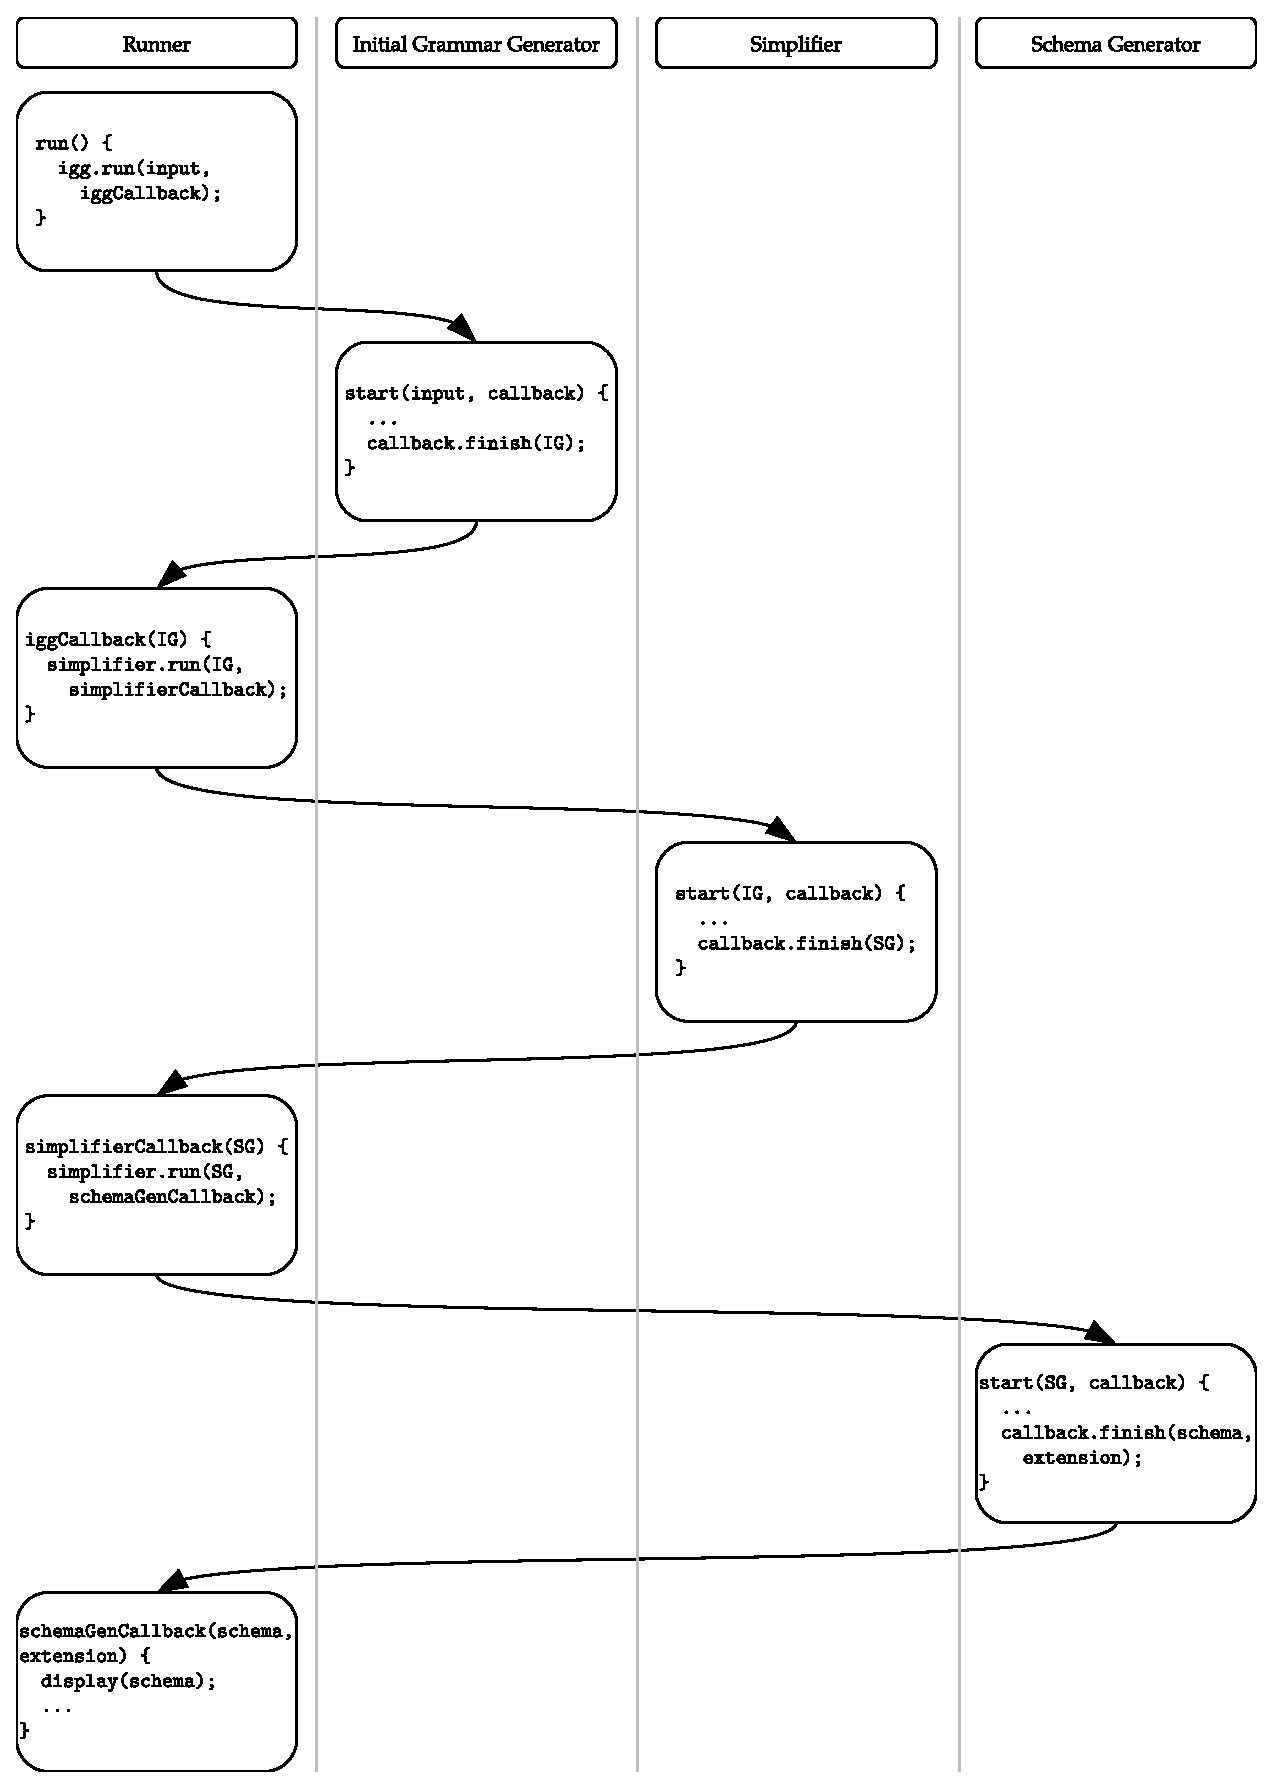
\includegraphics[scale=\myscale]{runner}
\caption{Runner} \label{runner}
\end{figure}
\begin{enumerate}
	\item Selected IGG's \code{start} is encapsulated with error/interruption handling and executed, passing \code{Input} and first callback as parameters.
	\item When IGG finishes, it invokes callback's \code{finish} method, passing the IG as parameter.
	\item This in turn causes \code{Runner} to encapsulate and execute Simplifier's \code{start}, passing IG from the first callback and the second callback as parameters.
	\item When Simplifier finishes, it invokes callback's \code{finish} method, passing the simplified grammar as parameter.
	\item This again causes \code{Runner} to encapsulate and execute SchemaGen's \code{start}, passing the simplified grammar from the second callback and the third callback as parameters.
	\item SchemaGen finishes and invokes the last callback's \code{finish}, passing the resulting schema and its extension as parameters.
	\item \code{Runner} receives the resulting schema and based on preferences, saves it to a file, displays it, etc.
\end{enumerate}

\subsection{Node metadata} \label{section_metadata}
To allow simple extensibility of rules, class \code{AbstractNamedNode} contains a string-addressed map called \code{metadata} that can contain arbitrary object values.

At the present, jInfer modules use the following metadata, all defined in \code{IGGUtils} class:
\begin{itemize}
	\item \code{from.xml}, filled in by \jmodule{BasicIGG} module: means that this rule was created (originates from) from a XML document.
	\item \code{from.schema}, filled in by \jmodule{BasicIGG} and \jmodule{XSDImporter} modules: means that this rule was created (originates from) from a schema.
	\item \code{from.query}, filled in by \jmodule{BasicIGG} and \jmodule{XSDImporter} modules: means that this rule was created from a query.
	\item \code{is.sentinel}, filled in by \jmodule{BasicIGG} and \jmodule{XSDImporter} modules: when importing XML document, one can build whole tree in memory (as in fig. \ref{xml_example}) and then construct list of rules from it (thus saving memory). With schema import however, one not only doesn't know right side of rule in advance (solved by stack in XML import), but right side can be defined anywhere in source file. To save complicated loading of whole schema, searching and pairing elements thorough rules, nodes on right side of rule are created empty - holding only name of node. Fact, that this node has no more information than it's name and position on right side of rule is denominated by labeling the node as sentinel.
	\item \code{required}, filled in by \jmodule{BasicIGG} and \jmodule{XSDImporter} modules: indicates that the attribute is required.
\end{itemize}
All of these metadata are of set/not set character (using \code{Boolean.TRUE} as value, but their presence effectively means "true").

\subsection{Capabilities} \label{section_capabilities}
From time to time, modules need a flow of certain information in completely opposite way to the usual inference: they need to know what the following module can or cannot do.

For this reason, inference modules extend the \code{Capabilities} interface defining a single method: \code{getCa\.pa\.bi\.li\.ties()}. This method returns a list of strings representing the abilities, or "capabilities" of this module.
An inference module can query the capabilities of the \emph{next} module in the inference chain by invoking the 
\begin{verbatim}
RunningProject.getNextModuleCaps()
\end{verbatim}
method to obtain the next module encapsulated in the \code{Capabilities} interface.

At the moment, only one capability is defined to be communicated across modules, more specifically between \jmodule{IGGenerator} and \jmodule{Simplifier}. This is \code{Capabilities.CAN\_HANDLE\_COMPLEX\_REGEXPS} meaning whether the \code{Simplifier} accepts more complicated regular expressions than simple concatenations of tokens on its input.

Example of Capabilities usage taken from \jmodule{XSDImporter} module:
\begin{verbatim}
// if the next module cannot handle complex regexps, help it by expanding our result
if (!RunningProject.getNextModuleCaps().getCapabilities()
             .contains(Capabilities.CAN_HANDLE_COMPLEX_REGEXPS)) { 
  // lookup expander
  final Expander expander = Lookup.getDefault().lookup(Expander.class);
  // return expanded
  return expander.expand(parser.getRules());
}
// return not expanded rules
return parser.getRules();
\end{verbatim}

\section{Platform view}
jInfer, being a NetBeans Platform application, is divided into multiple \emph{NetBeans Modules}. It is very important to understand that this division is in principle orthogonal to that naturally sketched in the previous chapters - theoretically, the whole jInfer could be contained in a single NB module, because the framework uses Lookups to locate logical modules. However, for the sake of organization, jInfer is split into several modules and most of the time there is a strong correlation between logical units of jInfer and its NB modules.

A short overview of these modules and their functions follows. To get a deeper understanding of any of them, please refer to its documentation. To get deeper understanding of how NBP modules work, their versions, dependencies etc, refer to \cite{modules_api}.

\noindent Base modules:
\begin{itemize}
	\item \jmodule{jInfer}: not a NBP module in fact, but rather a module suite - the ``root" NB project for the whole framework.
	\item \jmodule{Base}: contains common data structures, interfaces and utility logic shared across all other modules.
\end{itemize}

\noindent Inference modules:
\begin{itemize}
	\item \jmodule{Runner}: as described in the section \ref{section_runner}, this module encapsulates the inference process (including the fact that inference consists of 3 phases as described before). Most important class: \code{Runner}.
	\item \jmodule{BasicIGG}: this module contains an extensible implementation of \jmodule{IGGenerator}. Basic version handles all XML-typed input documents, DTD schemas and XPath queries. To find out more about the extensibility to handle other outputs, refer to \jmodule{BasicIGG}'s documentation.
	\item \jmodule{XSDImport}: demonstrating \jmodule{BasicIGG}'s extensibility, this is a base module for XSD input.
	\item \jmodule{XSDImportSAX}: XSD input handling using SAX parser.
	\item \jmodule{XSDImportDOM}: XSD input handling using DOM parser.
	\item \jmodule{TwoStepSimplifier}: a \jmodule{Simplifier} implementation. Implements \cite{ahonen} merging state algorithm with basic handling of attributes. Read the separated documentation of module.
	\item \jmodule{BasicDTDExporter}: this is a \jmodule{SchemaGenerator} implementation with output to DTD.
	\item \jmodule{BasicXSDExporter}: this is a \jmodule{SchemaGenerator} implementation with output to XSD.
\end{itemize}

\noindent Utility modules:
\begin{itemize}
	\item \jmodule{BasicRuleDisplayer}: module capable of displaying a grammar in a graphical way.
	\item \jmodule{TreeRuleDisplayer}: more advanced version of the former using \jmodule{JUNG}'s graphing capabilities.
	\item \jmodule{AutoEditor}: encapsulation of an interactive finite state automaton editor.
	\item \jmodule{JUNG}: wrapper module for the JUNG (see \cite{jung}).
	\item \jmodule{Options}: NBP specific: this module adds a jInfer category in NetBeans Options window.
	\item \jmodule{ProjectType}: NBP specific: this module defines a jInfer project type, along with its input and output files, settings etc.
	\item \jmodule{XPathFileType}: NBP specific: this module teaches NetBeans to recognize a \code{.xpath} file extension.
\end{itemize}
The dependencies between all the modules are summarized in figure \ref{module_deps}. Figure \ref{modules_inference} shows modules implementing the 3 main inference interfaces described in \ref{section_inference_process}.

\begin{figure}
	\centering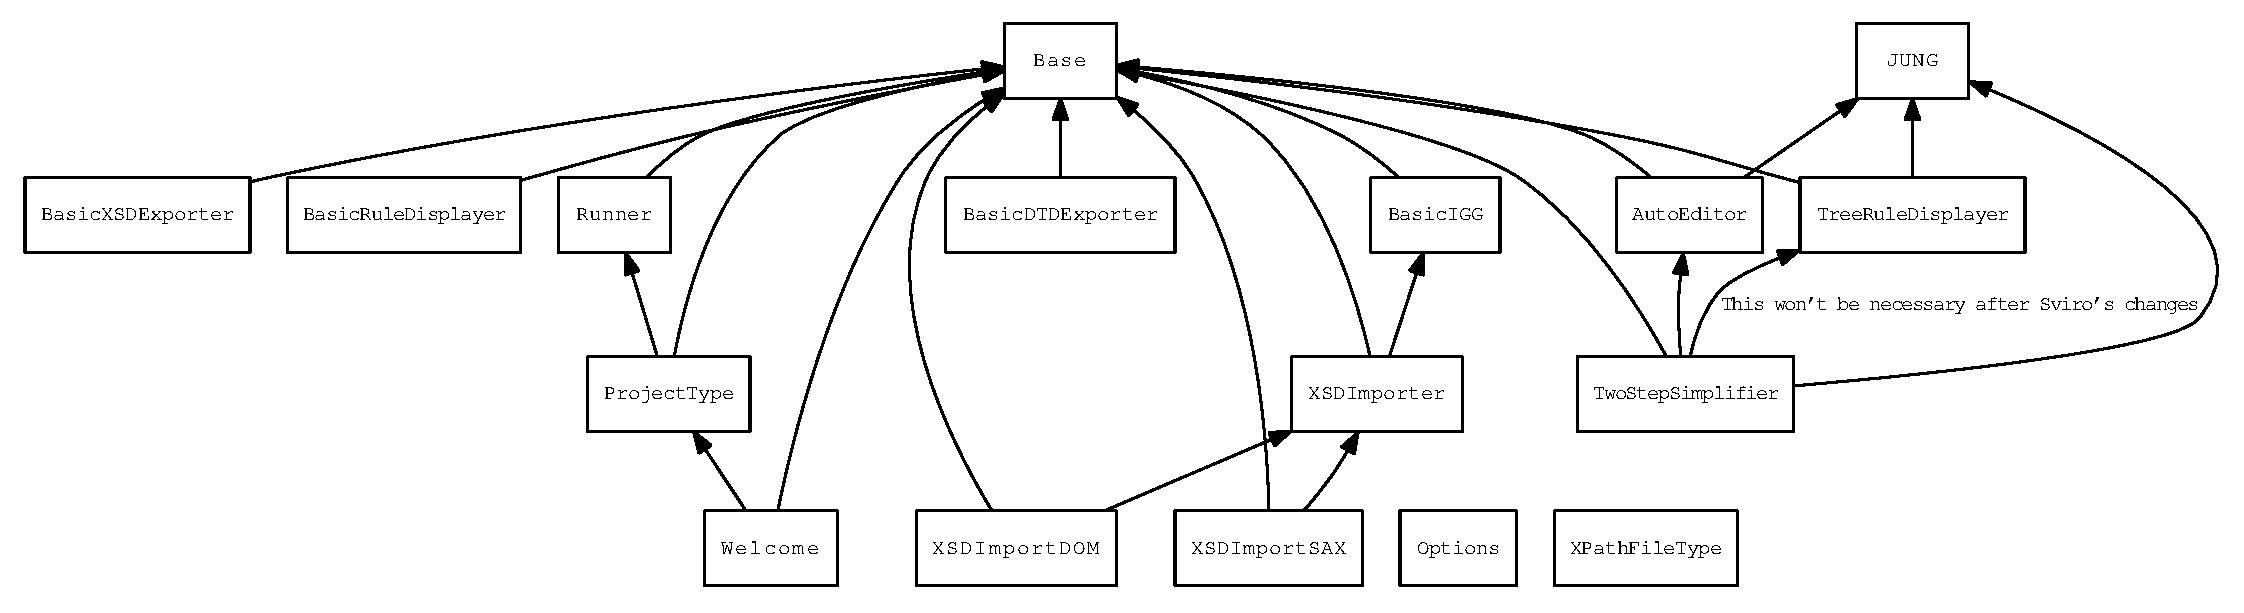
\includegraphics[scale=1]{module_deps}
	\caption{Module dependencies} \label{module_deps}
\end{figure}

\begin{figure}
	\centering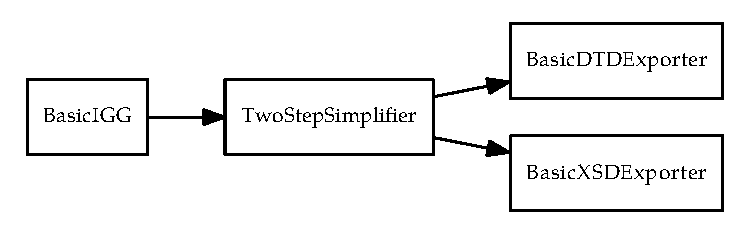
\includegraphics[scale=\myscale]{modules_inference}
	\caption{Inference modules in default jInfer} \label{modules_inference}
\end{figure}

\subsection{Lookups} \label{section_lookups}
\emph{Lookups} are a part of NBP API, a way to achieve late-binding between code based on this platform. An important notion is the one of a \emph{service provider}. This is a class implementing an interface, annotated in the following way (shown on an example from \jmodule{BasicDTDExporter}).
\begin{verbatim}
@ServiceProvider(service = SchemaGenerator.class)
public class SchemaGeneratorImpl implements SchemaGenerator {
  ...
\end{verbatim}
The \code{@ServiceProvider} annotation tells NBP that \code{SchemaGeneratorImpl} is to be registered among all providers of the \code{SchemaGenerator} service (or interface).

To look up a service provider, or all of them, one can use the \jmodule{Lookups} API in the following way.
\begin{verbatim}
Collection<SchemaGenerator> generators = Lookup.getDefault().lookupAll(SchemaGenerator.class);

for (SchemaGenerator g : generators) {
  System.out.println(g.getName());
}
\end{verbatim}
Call to \code{Lookup.getDefault().lookupAll()} will return a collection of all service providers registered to be providing the \code{SchemaGenerator} interface. This collection can be walked in some way, and on one or more of service providers methods can be called. We didn't have to actually bind providers to logic that uses their services, NB Platform took care of this for us.

See \cite{lookup_api} as the official documentation to lookup API.

\subsection{Factory pattern}
\begin{figure}
  \centering
	\subfigure[Same instance of class returned by NetBeans in two successive inference runs]
	{
	  \centering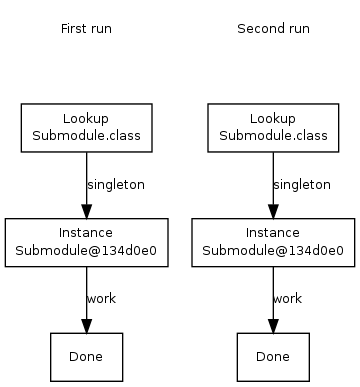
\includegraphics[scale=\myscale]{factory_pattern1}
    \label{factory_pattern1}
  }
	\subfigure[Factory solution of singleton lookup class problem]
	{
	  \centering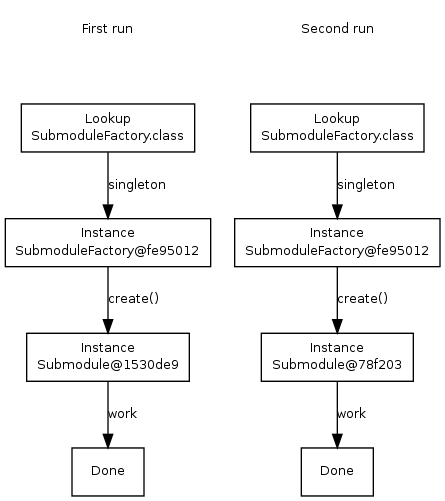
\includegraphics[scale=\myscale]{factory_pattern2}
    \label{factory_pattern2}
  }
\end{figure}
At this point it is important to understand that when using lookups this way, all service providers are kept as singletons. 
We ilustrate this behaviour on \ref{factory_pattern1}, user runs inference first time, classes are looked up and used.
When user clicks run button again, and same instances of classes are returned by lookups.

In case a provider needs to change its state during providing the service (and needs to be ``fresh'' each time it is retrieved), there are two solutions:
\begin{itemize}
	\item force each service providing class (submodule), to implement
some sort of cleanup method, that would restart it into fresh state and make it ready to use by another 
inference run,
	\item or create new instances of stateful classes in each inference run and make service providing classes (those which NetBeans return by lookups) factories.
\end{itemize}
We decided for the latter approach (as ilustrated on fig. \ref{factory_pattern2}
It enables us not only to produce fresh class instance in each inference run, but also factory classes implement obligatory
module methods such as \code{getName}, \code{getDescription} and so on, which are really same in each inference run.
Each submodule is then defined by (at least) two interfaces.
One is the factory interface, like this one (example from \jmodule{TwoStepSimplifier}:
\begin{verbatim}
public interface AutomatonSimplifierFactory extends 
                     NamedModule, Capabilities, UserModuleDescription {
  <T> AutomatonSimplifier<T> create();
}
\end{verbatim}
Second is worker interface, in the example it is \code{AutomatonSimplifier<T>} interface.

This pattern is used thorough jInfer modules to divide module into submodules.

\subsection{Tokens}
An important topic related to NB modules and their dependencies is a notion of \emph{tokens}. Imagine a situation where module \emph{M} needs \emph{someone} else to provide a certain service \emph{S}, but doesn't care who will that be. It cannot declare a direct dependency on a module containing this service provider, because it might not know such a module. Instead, \emph{M} declares a \emph{required token}. Any module providing \emph{S} will declare a \emph{provided token}, which is a simple string (usually fully qualified Java name of the interface representing \emph{S}). Later, NBP will make sure that \emph{M} can be installed in the platform only if there is at least one module providing that specific token.

jInfer uses tokens in the following way: \jmodule{Runner}, as the module encapsulating the inference process, and \jmodule{ProjectType} as an encapsulation of jInfer projects both require the following 3 tokens.
\begin{itemize}
	\item \code{cz.cuni.mff.ksi.jinfer.base.interfaces.inference.IGGenerator}
	\item \code{cz.cuni.mff.ksi.jinfer.base.interfaces.inference.SchemaGenerator}
	\item \code{cz.cuni.mff.ksi.jinfer.base.interfaces.inference.Simplifier}
\end{itemize}
All inference modules declare their respective token as provided. This way it is ensured that jInfer will run only if there is at least one implementation of each of the inference modules, regardless of the implementation itself.

%\nocite{*}
\newpage
\bibliographystyle{alpha}
\bibliography{literature}

\end{document}
